\paragraph{(a)}
El An\'alisis de Componentes Principales (PCA) consiste en una transformaci\'on lineal ortogonal que transforma los datos
a un nuevo sistema coordenado de tal forma que este nuevo sistema queda determinado por \textit{componentes principales}
que est\'an no correlacionados entre s\'i (son ortogonales), pero que tienen m\'axima correlaci\'on con las mediciones.
Esta transformaci\'on consigue que el primer componente principal tenga la mayor posible varianza, el siguiente componente segunda
mayor varianca y as\'i sucesivamente. Para esto, los datos se pre-procesan y luego se ejecuta SVD. 
\\
M\'as espec\'ificamente, suponiendo que $X$ es una matriz que contiene en cada fila mediciones de un experimento y que al cambiar de fila
lo que cambia es el \textit{feature} del experimento, calculamos la media $\bar{x}$ como 
\[\bar{x}_j = \frac{1}{n}\sum_{i=1}^nX_{ij} \]
y la matriz promedio la definimos como 
\[\bar{X} = h\cdot\bar{x}^t \]
donde $h$ es un vector que cumple $h_i = 1$ para $i=1,\ldots,n$. Se define la matriz promedio-substra\'ida $B$ como
\[ B = X-\bar{X} \]
y la matriz de covarianca de las filas de $B$ es dada por
\[ C = \frac{1}{n-1}B^*B \]

Con esto, la relaci\'on entre PCA y SVD se puede visualizar m\'as claramente: el componente principal $u_1$ es dado por
\[ u_1 = \arg \max_{||u_1||=1} u_1^*B^*Bu_1 \]
el cual corresponde al vector propio de $B^*B$ correspondiente al mayor valor propio. De aqu\'i es claro que $u_1$ es el vector singular 
izquierdo de $B$ correspondiente al m\'as grande valor singular. Luego, los componentes principales se 
encuentran  aplicando descomposici\'on por valores propios a la matriz $C$.\\
\paragraph{(b)}
Se eligi\'o el ejemplo de \textit{Ovarian cancer data}. La idea del ejemplo es estudiar la informaci\'on
gen\'etica de 216 pacientes, de los cuales 121 tienen c\'ancer de ovario y 95 no. Para cada paciente
hay un vector de datos que contiene la expresi\'on gen\'etica de 4000 genes. Los datos de expresi\'on gen\'etica tienen la complejidad de ser de alta dimensi\'on (aqu\'i, dimensi\'on se refiere a la cantidad de 
atributos que un conjunto de datos tiene). Una sola persona tiene millones de posibles combinaciones gen\'eticas y esto provoca
que la informaci\'on gen\'etica de los pacientes tengan alta correlaci\'on, al punto que la informaci\'on de un paciente se traslapa
con otros. Para poder visualizar patrones y correlaciones
en datos de alta dimensi\'on como \'estos el uso de PCA se vuelve fundamental.\\
\paragraph{(c)}
El c\'odigo se muestra a continuaci\'on.
\lstinputlisting[language=MATLAB]{../codigo/ejer7.m}
El resultado que se obtiene es el gr\'afico de la siguiente figura.
\begin{figure}[H]
   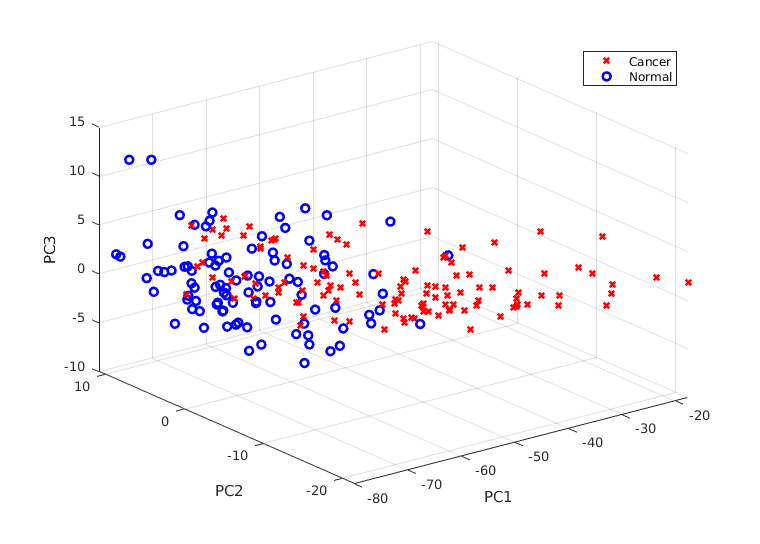
\includegraphics[width=\textwidth]{ejer7c.png}
   \centering
   \caption{Gr\'afico usando PCA en datos de pacientes con c\'ancer y pacientes sanos.}
\end{figure}

Se observa que los datos de  personas con c\'ancer tienden a dispersarse m\'as que las personas sin c\'ancer.
